\begin{figure*}
    \centering
    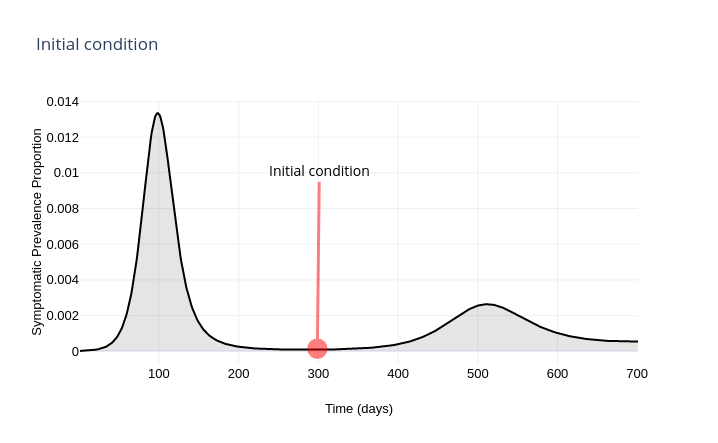
\includegraphics[scale=0.5, keepaspectratio]{figs/InitialCondition}
    \caption[Initial condition]{
        Initial condition scheme. We assume a positive
        prevelance. Forreference, at the date of write this manuscript,
        prevalence in CDMX is
        arounn \SI{16000}{cases}, see
        \href{https://plotly.com/~sauld/36/}{https://plotly.com/~sauld/36/} to
        display a electronic viewer.}
        \label{fig:initialcondition}
\end{figure*}

\begin{figure*}[tbh]
    \centering
    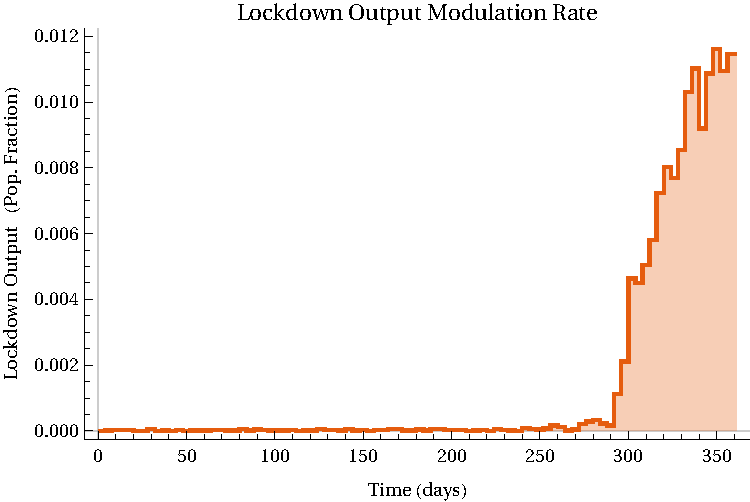
\includegraphics[width=0.7\linewidth]{figs/lockdown_control_signal}
    \caption[Lockdown modulation signal.]{Lockdown modulation signal.}
    \label{fig:lockdowncontrolsignal}
\end{figure*}

\begin{figure}
    \centering
    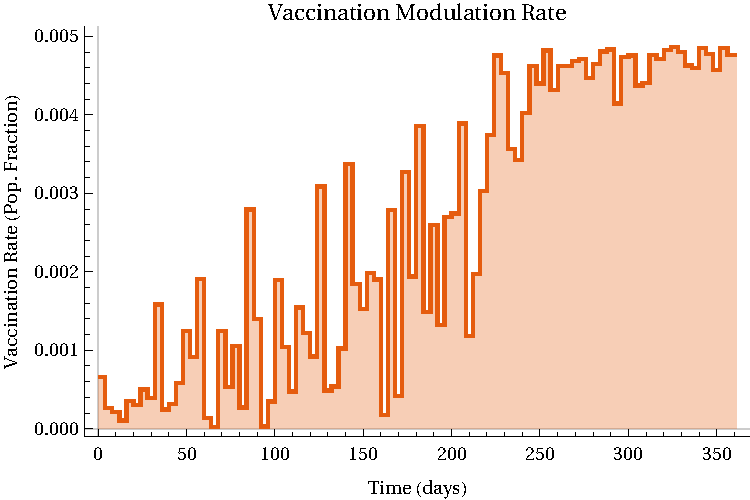
\includegraphics[width=0.7\linewidth]{figs/Vaccination_control_signal}
    \caption[Vaccination rate modulation.]{Vaccination rate modulation.}
    \label{fig:vaccinationcontrolsignal}
\end{figure}

\begin{figure}[tbh]
    \centering
    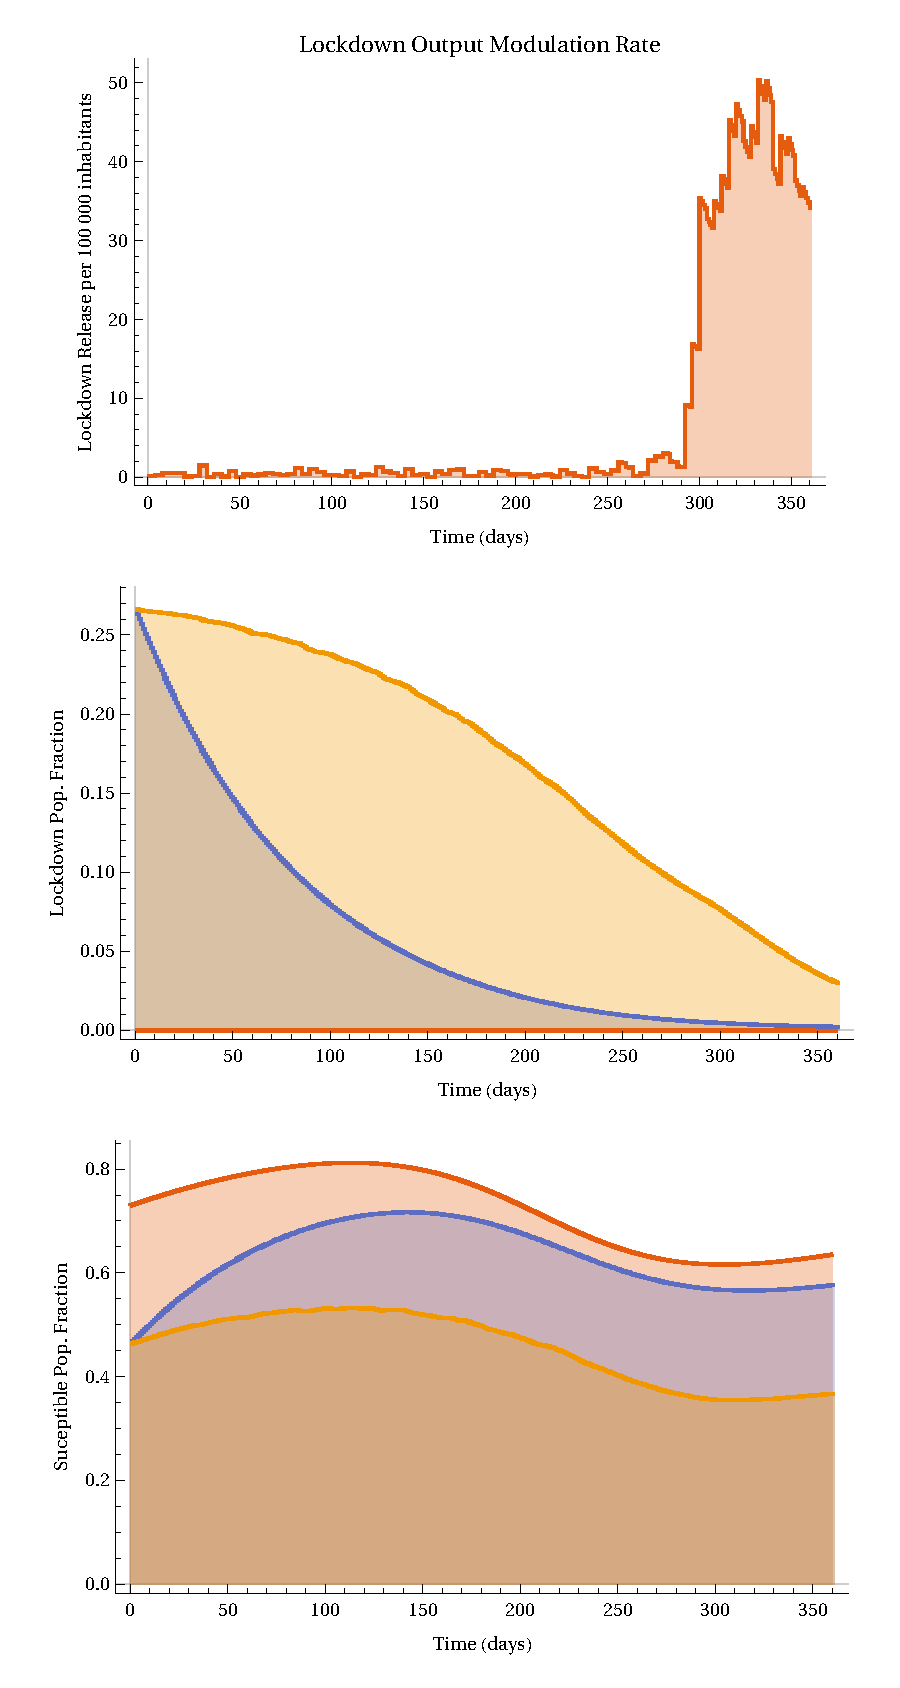
\includegraphics[width=1.0\linewidth]{figs/LockdownEffect}
    \caption{Modulation lock down release.}
    \label{fig:lockdowneffect}
\end{figure}
